%% Encoding: ISO8859-1 %%

\section{Grundlagen}

\frame{
\frametitle{Grundlagen}
    \begin{itemize}
        \item token basierte Schaltkreise (Bsp. Petri Netze)
        \item token pass Schaltkreise
        \item nicht polare token pass Brown'sche Schaltkreise
    \end{itemize}
}

%---------------------------------------------------------------------

\frame{
    \frametitle{Token basierte Schaltkreise}
    \begin{itemize}
        \item Signal als Token 
        \item asynchron (kein Takt)
    \end{itemize}

    \begin{figure}   
        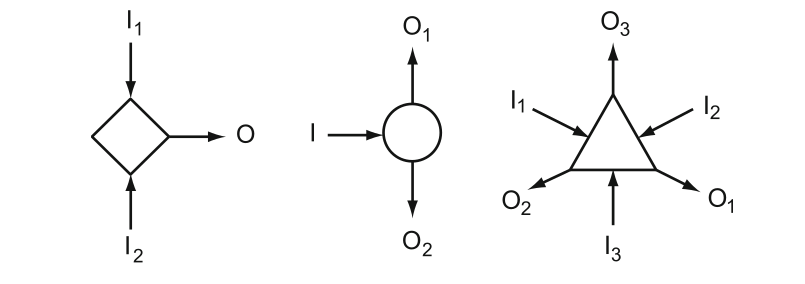
\includegraphics[width=7cm]{bilder/tokenBased.png}
        \caption{Merge, Fork und Tria sind Schaltkreisprimitive}
    \end{figure}
}

%---------------------------------------------------------------------

\frame{
    \frametitle{Token pass Schaltkreise}
    \begin{itemize}
        \item Einschr\"ankungen von token basiert
        \item Anzahl der Tokens immer gleich
        \item Tokens verlassen Kabel nicht
    \end{itemize}
   
    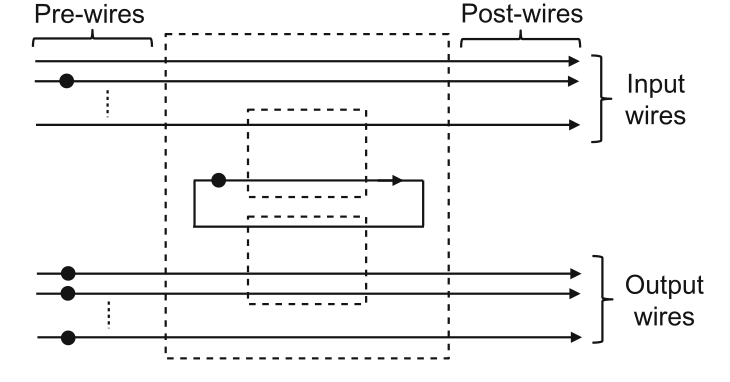
\includegraphics[width=5cm]{bilder/TokenPassScheme.png}
}    

%---------------------------------------------------------------------

\frame{
    \frametitle{Brown'sche Schaltkreise}
        \begin{itemize}
            \item Tokens k\"onnen sich frei bewegen 
            \item Vergleich Brown'sche Molekularbewegung 
            \item Verz\"ogerungen beeinflussen nicht Korrektheit der 
                Berechnung
        \end{itemize}


}

%---------------------------------------------------------------------

\frame{
    \frametitle{T-Element}
    \begin{minipage}{0.45\textwidth}
        \begin{itemize}
            \item Grundbaustein
            \item 
        \end{itemize}
    \end{minipage}\hfill

    \begin{minipage}{0.45\textwidth}
         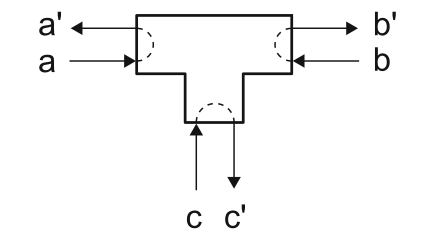
\includegraphics[width=6cm]{bilder/T_Element.png}
    \end{minipage}\hfill

}

%---------------------------------------------------------------------

\frame{
    \frametitle{\"Aquivalenz von token basiert und token pass}
    \centering
    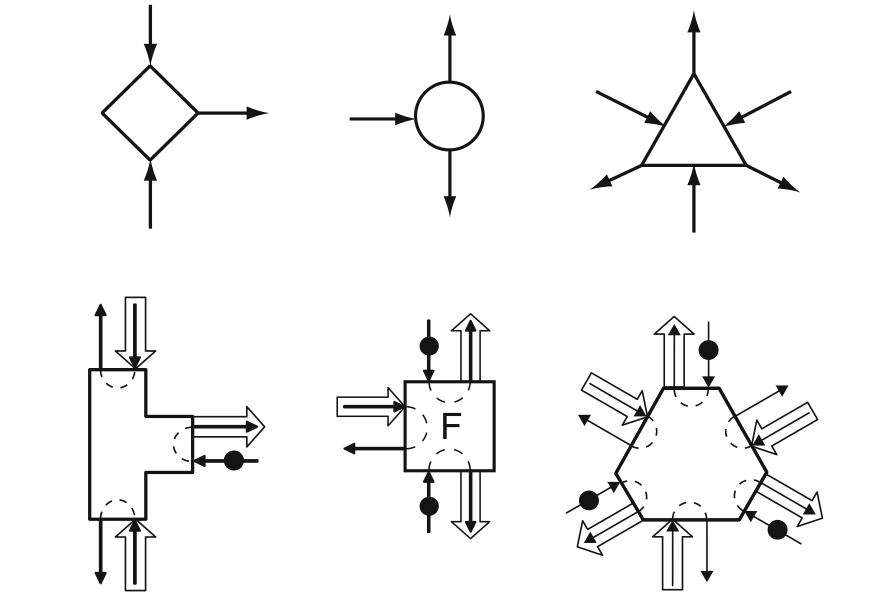
\includegraphics[width=8cm]{bilder/BasedToPass.png}

}

%---------------------------------------------------------------------

\frame{
    \frametitle{\"Aquivalenz von token basiert und token pass}
    \begin{figure}
        \begin{minipage}{0.45\textwidth}
            \centering
            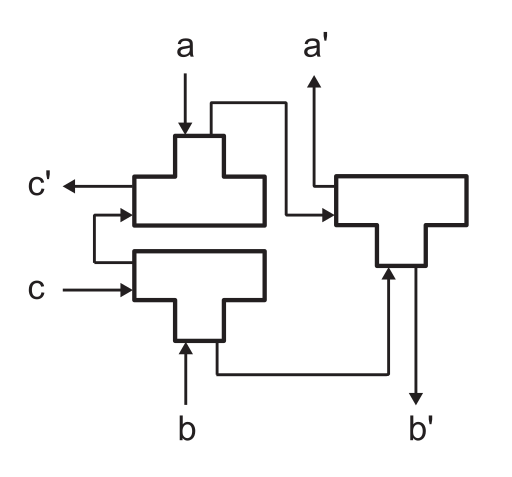
\includegraphics[width=5cm]{bilder/TP_Fork.png}
            \caption{Fork aus T-Elementen}
        \end{minipage}\hfill
        \begin{minipage}{0.45\textwidth}
            \centering
            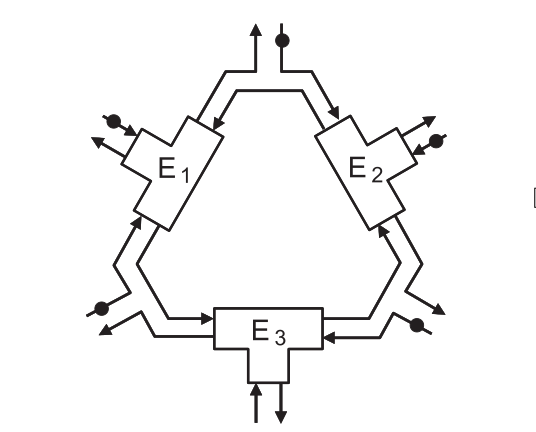
\includegraphics[width=5cm]{bilder/TP_Tria.png}
            \caption{Tria aus T-Elementen}
        \end{minipage}\hfill
    \end{figure}
}

%--------------------------------------------------------------------
\frame{
    \frametitle{\"Aquivalenz von token basiert und token pass}
    T-Element ist Schaltkreisprimitiv f\"ur brown'sche token pass 
    Schaltkreise 
}

%--------------------------------------------------------------------
%---------------------------------------------------------------------

\section{1-Bit Speicher}
%TODO Funktionsweise auf jeden Fall von nicht polarem, aber 
% soll ich auch das polare erklären ???
%für bilder die abläufe aus dem Paper benutzen


%---------------------------------------------------------------------
%---------------------------------------------------------------------

\section{UND-Gatter} 



%---------------------------------------------------------------------
%---------------------------------------------------------------------


\section{Ausblick} 




